\documentclass{ximera}

\title{Kleinste kwadraten benadering}
\author{Mila Vervoort}
\license{CC: 0}         % replace with an appropriate license, or set it in xmPreamble

\begin{document}
\begin{abstract}
    Kleinste kwadraten benadering
\end{abstract}
\maketitle
\label{xim:Integrale analysemethode}

\section*{Kleinste kwadraten benadering}
\label{Kleinste kwadraten benadering}

\subsection*{Algemeen principe}

Bij de integrale en diffenrentiële analysemethode, de methode der beginsnelheden en de methode der halfwaardetijden worden de kinetische parameters op een eenvoudige sequentiële manier bepaald. Deze methoden zijn echter vooral geschikt wanneer slechts één of twee parameters moeten worden geschat. \\
In de praktijk zijn reactiesnelheden vaak complexer van aard en afhankelijk van meerdere parameters. In dat geval is het vaak beter om de kinetische parameters gelijktijdig te bepalen aan de hand van een hele reeks experimenten. 
Beschouw bijvoorbeeld de reactiesnelheid:

\[
- \frac{dC_A}{dt}=-R_A=kC_A^nC_B^m,
\]
waarin de onbekende parameters de snelheidsconstante $k$ en de reactieordes $n$ en $m$ zijn.

Deze vergelijking kan herschreven worden zodat we een lineair model krijgen:

\[
\underbrace{\ln\!\left(-\frac{dC_A}{dt}\right)}_{y}
=
\underbrace{\ln k}_{a_0}
+
\underbrace{n}_{a_1}\ln C_A
+
\underbrace{m}_{a_2}\ln C_B.
\]

Met

\[
x_1=\ln C_A,
\qquad
x_2=\ln C_B,
\]

kunnen we dit schrijven als

\[
y=a_0+a_1x_1+a_2x_2.
\]

Het bekomen model is lineair in de onbekende parameters, maar bevat nu twee onafhankelijke variabelen ($x_1$ en $x_2$). De parameters kunnen daarom niet langer grafisch worden bepaald zoals bij de vorige methoden, maar moeten gelijktijdig uit alle meetgegevens worden geschat.

Bovendien bevatten experimentele meetgegevens altijd een zekere meetfout. Hierdoor zal geen enkele combinatie van parameters de experimentele gegevens exact beschrijven.

De centrale vraag wordt dan:

\begin{center}
Welke parameterwaarden zorgen ervoor dat het kinetische model de experimentele meetgegevens zo goed mogelijk beschrijft?
\end{center}

Om deze vraag te beantwoorden gebruikt men de \textbf{kleinste kwadraten benadering} (\textit{Least Squares Approximation}).

\subsection*{Theoretische afleiding van de methode}

Veronderstel dat we $N$ experimenten uitvoeren. Voor elk experiment $j$
($j=1,\ldots,N$) meten we de concentraties $C_A$ en $C_B$ en bepalen we de
reactiesnelheid. Na de logaritmische transformatie beschikken we over de
gegevens

\[
(x_{1,j},x_{2,j},y_j),
\qquad j=1,\ldots,N.
\]

Voor een gegeven keuze van de parameters $a_0$, $a_1$ en $a_2$ voorspelt het
lineaire model de waarde

\[
\hat{y}_j
=
a_0+a_1x_{1,j}+a_2x_{2,j}.
\]

\textit{(De notatie $\hat{y}$ wordt gebruikt om aan te geven dat dit de door het model voorspelde waarde is, in tegenstelling tot de experimenteel gemeten waarde $y$.)}

Voor elke andere keuze van de parameters krijgen we een andere voorspelling. De parameters van het model bepalen dus rechtstreeks hoe goed het model de experimentele gegevens beschrijft. De kleinste-kwadratenmethode zal daarom niet zomaar de waarden van $a_0$, $a_1$ en $a_2$ kiezen, maar zoekt specifiek naar de combinatie die de
beste overeenkomst geeft tussen het model en de experimenten.

De experimentele waarde $y_j$ en de modelvoorspelling $\hat{y}_j$ zullen in het
algemeen niet gelijk zijn:

\[
y_j \neq \hat{y}_j
\]

Het model maakt dus voor elke meetwaarde een voorspelling, maar deze voorspelling
wijkt door meetfouten en modelonnauwkeurigheden af van het experiment.

Het verschil tussen de experimentele waarde en de modelwaarde noemen we het
\textbf{residu}:

\[
e_j
=
y_j-\hat{y}_j.
\]

Voor een ideaal model dat de reactiesnelheidsvergelijking perfect beschrijft, zouden alle residuen gelijk zijn aan nul.

De grootte van deze residuen hangt dus af van de gekozen waarden van de parameters. Door de parameters van het model te veranderen, verandert immers ook de voorspelde waarde $\hat{y}_j$ en bijgevolg ook het residu.

De optimale parameters zijn deze waarvoor $S$ minimaal wordt.

Men zou kunnen proberen de residuen eenvoudig op te tellen,

\[
\sum_{j=1}^{N}e_j,
\]

maar dit is geen goede maat voor de kwaliteit van de benadering.
Positieve en negatieve residuen kunnen elkaar immers opheffen, waardoor een
slechte benadering toch een kleine som kan opleveren.

Daarom beschouwen we de \textbf{som van de gekwadrateerde residuen}

\[
S
=
\sum_{j=1}^{N}e_j^2.
\]

Door de residuen te kwadrateren zijn alle bijdragen positief en krijgen grote
afwijkingen bovendien een groter gewicht dan kleine afwijkingen.

Het principe van de kleinste-kwadratenmethode kan daarom schematisch worden weergegeven als:
\[
(a_0,a_1,a_2)
\longrightarrow
\hat{y}_j
\longrightarrow
e_j=y_j-\hat{y}_j
\longrightarrow
S=\sum_j e_j^2
\]

Invullen van de uitdrukking voor het residu levert

\[
S(a_0,a_1,a_2)
=
\sum_{j=1}^{N}
\left(
y_j-a_0-a_1x_{1,j}-a_2x_{2,j}
\right)^2.
\]

De methode van de kleinste kwadraten bestaat erin de waarden van
$a_0$, $a_1$ en $a_2$ te bepalen waarvoor deze som minimaal is.

Wiskundig schrijven we dit als

\[
\boxed{
\min_{a_0,a_1,a_2}
S(a_0,a_1,a_2).
}
\]

De functie $S$ is een functie van drie onbekende parameters. Elke keuze van
$a_0$, $a_1$ en $a_2$ levert een andere waarde voor $S$. We zoeken dus de
parametercombinatie waarvoor de som van de gekwadrateerde residuen zo klein
mogelijk is.

Bij een functie van één variabele wordt een minimum gevonden door de afgeleide gelijk te stellen aan nul. Op het minimum verandert de functie immers niet meer wanneer de onafhankelijke variabele een kleine verandering ondergaat.

Omdat $S$ afhankelijk is van drie parameters, moeten we controleren of er geen verbetering mogelijk is door één van deze parameters afzonderlijk te wijzigen. Daarom moet de helling van $S$ in elke mogelijke richting nul zijn:

\[
\frac{\partial S}{\partial a_0}=0,
\qquad
\frac{\partial S}{\partial a_1}=0,
\qquad
\frac{\partial S}{\partial a_2}=0.
\]

We werken deze partiële afgeleiden één voor één uit.

Voor de afgeleide naar $a_0$ bekomen we
\[0 = \frac{\partial S}{\partial a_0} 
= \sum_{j=1}^{N}2\left[y_j-(a_0+a_1x_{1,j}+a_2x_{2,j})\right](-1).
\]

Analoog volgt voor de afgeleiden naar $a_1$ en $a_2$

\[0 = \frac{\partial S}{\partial a_1} 
= \sum_{j=1}^{N} 2\left[y_j-(a_0+a_1x_{1,j}+a_2x_{2,j})\right](-1)x_{1,j},\]

\[0 = \frac{\partial S}{\partial a_2} 
= \sum_{j=1}^{N}2\left[y_j-(a_0+a_1x_{1,j}+a_2x_{2,j})\right](-1)x_{2,j}.
\]


De factoren $2$ en $-1$ zijn verschillend van nul en kunnen bijgevolg worden
weggelaten. Na het uitwerken van de haakjes en het groeperen van gelijke termen
bekomen we het volgende stelsel van drie lineaire vergelijkingen:

\[
\sum_{j=1}^{N} y_j
=
a_0N
+
a_1\sum_{j=1}^{N}x_{1,j}
+
a_2\sum_{j=1}^{N}x_{2,j},
\]

\[
\sum_{j=1}^{N}y_jx_{1,j}
=
a_0\sum_{j=1}^{N}x_{1,j}
+
a_1\sum_{j=1}^{N}x_{1,j}^2
+
a_2\sum_{j=1}^{N}x_{1,j}x_{2,j},
\]

\[
\sum_{j=1}^{N}y_jx_{2,j}
=
a_0\sum_{j=1}^{N}x_{2,j}
+
a_1\sum_{j=1}^{N}x_{1,j}x_{2,j}
+
a_2\sum_{j=1}^{N}x_{2,j}^2.
\]

Deze vergelijkingen worden de \textbf{normaalvergelijkingen} genoemd. Ze vormen
een stelsel van drie lineaire vergelijkingen met de drie onbekenden $a_0$, $a_1$ en $a_2$. Door dit stelsel op te lossen verkrijgen we de regressiecoëfficiënten van het lineaire model.

\begin{example} \textbf{Een rechte fitten met de kleinste-kwadratenmethode} 
In de hoofdstukken over de integrale en differentiële analysemethode werd eenrechte door de experimentele meetpunten gefit met behulp van de Python-functie \texttt{polyfit}. 

Deze functie gebruikt achterliggend de methode van de kleinste kwadraten om de coëfficiënten van de best passende rechte te bepalen. We bekijken nu hoe hetzelfde resultaat stap voor stap bekomen kan worden met de afleiding uit de vorige paragraaf.

Beschouw bijvoorbeeld de volgende meetgegevens (dit zijn de gegevens van oefening 2 op de integrale analysemethode):
\[
\begin{array}{c|ccccc}
x = t~(\mathrm{min}) &0&1&2&3&4\\
\hline
y = -\ln\left(\frac{C_A-C_{A,eq}}{C_{A0}-C_{A,eq}}\right)&0.00&0.60&1.20&1.90&2.66
\end{array}
\]

In Python werd de regressierechte bepaald met
\begin{verbatim}
a, b = np.polyfit(x, y, 1)
y_fit = a*np.array(x) + b
\end{verbatim}

De functie \texttt{np.polyfit()} voert deze optimalisatie automatisch uit. Achterliggend worden de parameters $a_0$ en $a_1$ bepaald waarvoor de som van de gekwadrateerde afwijkingen minimaal wordt:

\[
S=\sum_j(y_j-(a_0+a_1x_j))^2
\]

De gebruiker hoeft dus de normaalvergelijkingen niet zelf op te lossen.

We bekijken nu hoe dezelfde rechte bekomen wordt met de methode van de
kleinste kwadraten.\\

Omdat we slechts één onafhankelijke variabele hebben, schrijven we het model als
\[
y=a_0+a_1x,
\]
waarbij
\[x=t.\]

De som van de gekwadrateerde residuen wordt
\[
S(a_0,a_1) = \sum_{j=1}^{N}\left(y_j-a_0-a_1x_j\right)^2.
\]

Om het minimum van deze functie te bepalen stellen we de partiële afgeleiden gelijk aan nul.\\
Dit leidt tot de twee normaalvergelijkingen
\[\sum y_j = Na_0 + a_1\sum x_j,\]
\[\sum x_jy_j = a_0\sum x_j + a_1\sum x_j^2. \]

We berekenen nu eerst alle benodigde sommen.

\[
\sum x_j = 10,  
\sum y_j = 6.36, 
\sum x_j^2 = 30,
\sum x_jy_j = 19.34
\]

Invullen in de normaalvergelijkingen geeft

\[
6.36 = 5a_0 + 10a_1,
\]

\[19.34 = 10a_0 + 30a_1.
\]

We lossen dit stelsel op.
Uit de eerste vergelijking volgt

\[ a_0 = \frac{6.36-10a_1}{5}.\]

Invullen in de tweede vergelijking geeft
\[19.34 = 10\left( \frac{6.36-10a_1}{5}\right)+30a_1,\]
of
\[19.34 = 12.72-20a_1+30a_1.\]

Hieruit volgt
\[a_1 =0.662.\]
\[a_0 = -0.052.\]


De regressierechte wordt dus

\[
\boxed{
y=-0.052+0.662\,t.
}
\]

Deze waarden komen (op afrondingsverschillen na) overeen met het resultaat berekend met \texttt{np.polyfit(x,y,1)}.

\begin{figure}[h!]
\centering
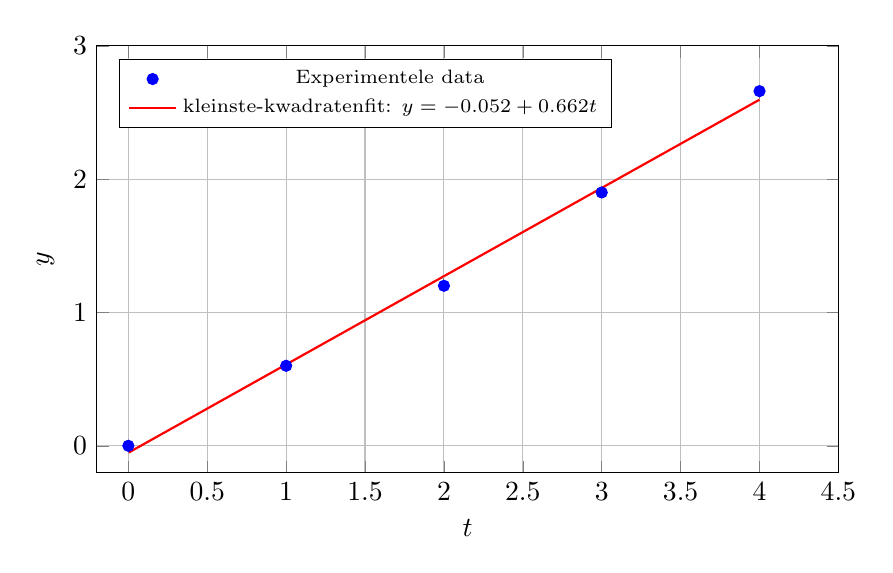
\begin{tikzpicture}
\begin{axis}[
    width=11cm,
    height=7cm,
    xlabel={$t$},
    ylabel={$y$},
    xmin=-0.2,
    xmax=4.5,
    ymin=-0.2,
    ymax=3,
    grid=major,
    legend style={
        at={(0.03,0.97)},
        anchor=north west,
        font=\scriptsize
    }
]

% Meetpunten
\addplot[
    only marks,
    mark=*,
    mark size=2pt,
    blue
]
coordinates {
    (0,0)
    (1,0.60)
    (2,1.20)
    (3,1.90)
    (4,2.66)
};
\addlegendentry{Experimentele data}

% Regressierechte y=-0.052+0.662t
\addplot[
    red,
    thick,
    domain=0:4
]
{-0.052+0.662*x};

\addlegendentry{
    kleinste-kwadratenfit:
    $y=-0.052+0.662t$
}

% Residuen tekenen
\addplot[
    dashed,
    gray
]
coordinates {
    (0,0) (0,-0.052)
};

\addplot[
    dashed,
    gray
]
coordinates {
    (1,0.60) (1,0.610)
};

\addplot[
    dashed,
    gray
]
coordinates {
    (2,1.20) (2,1.272)
};

\addplot[
    dashed,
    gray
]
coordinates {
    (3,1.90) (3,1.934)
};

\addplot[
    dashed,
    gray
]
coordinates {
    (4,2.66) (4,2.596)
};
\end{axis}
\end{tikzpicture}
\caption{Lineaire regressie van de meetgegevens met de kleinste-kwadratenmethode. 
De verticale afstanden tussen de meetpunten en de regressierechte stellen de residuen voor.}
\label{fig:kleinste_kwadraten_rechte}
\end{figure}

De figuur toont grafisch wat de kleinste-kwadratenmethode probeert te bereiken:
niet noodzakelijk een rechte die door alle punten gaat, maar een rechte waarvoor
de totale afwijking tussen model en experiment minimaal is.

\end{example}

\subsection*{Praktische uitvoering}

Hoewel de normaalvergelijkingen analytisch kunnen worden opgelost, gebeurt dit in
de praktijk vrijwel nooit met de hand. Bij een groot aantal experimenten of een
groter aantal onbekende parameters wordt het oplossen van deze vergelijkingen
immers snel omslachtig.

Daarom worden regressieproblemen tegenwoordig vrijwel altijd numeriek opgelost
met behulp van software zoals Python, MATLAB of Excel. Deze programma's
implementeren efficiënte algoritmen die de kleinste-kwadratenoplossing
automatisch bepalen.

Het basisprincipe blijft echter hetzelfde als bij de analytische afleiding:
er wordt gezocht naar de parameterwaarden waarvoor de som van de
gekwadrateerde residuen minimaal is.

Bij eenvoudige lineaire modellen, zoals

\[
y=a_0+a_1x,
\]

kunnen de normaalvergelijkingen rechtstreeks worden opgesteld en opgelost.
Bij complexere modellen, zoals kinetische reactiesystemen, is dit meestal niet
meer praktisch mogelijk. De onbekende parameters zijn dan vaak verweven in een
systeem van differentiaalvergelijkingen.

In dat geval wordt gebruikgemaakt van een numerieke optimalisatieprocedure. De
software probeert verschillende waarden van de onbekende parameters uit en
berekent telkens hoe goed het model de experimentele gegevens beschrijft.

Hiervoor gebruiken we in Python de functie
\texttt{least\_squares()} uit de bibliotheek
\texttt{scipy.optimize}.
Deze functie bevat het optimalisatie-algoritme, maar kent zelf niets van het
onderliggende kinetische model. De gebruiker moet daarom drie zaken definiëren:

\begin{enumerate}
    \item een model dat, voor een gegeven set parameters, voorspellingen maakt;
    \item een functie die het verschil tussen model en experiment berekent
    (de residuen);
    \item een eerste schatting van de onbekende parameters.
\end{enumerate}

De functie \texttt{least\_squares()} past vervolgens de parameters automatisch
aan totdat de som van de gekwadrateerde residuen minimaal is:

\[
S=\sum_i e_i^2
\]

waarbij

\[
e_i=y_{\text{model},i}-y_{\text{experiment},i}.
\]

In de volgende sectie bekijken we hoe deze werkwijze praktisch wordt toegepast
op een kinetisch reactiesysteem met behulp van Python.

\subsection*{Toepassingen}


\end{document}